\documentclass[twoside,colorbacktitle,accentcolor=tud6a]{tudexercise}
\usepackage{ngerman}

\usepackage{caption}                    % enumerated captions in figures, etc.
\usepackage{subcaption}                 % subcaptions for subfigures
\usepackage{hyperref}

\newcommand{\unit}[1]{{\rm\,#1}}
 

\title{Notes of  SDK \\Asctec HL Processor}
\subtitle{\today}
%\subsubtitle{Menmber: }
\renewcaptionname{ngerman}{\sectionname}{}
\usepackage{graphicx} 

\usepackage{indentfirst}
\setlength{\parindent}{2ex}


\begin{document}
\renewcommand{\figurename}{Figure.} 	
\setcounter{section}{0}
\maketitle
  \section{How to use the changed SDK code}
 If we copy the SDK code to another PC(e.g. git pull from github),we can not import the project in the Asctec SDK, it seems that it can only be imported from archive file. It has been tested, when we follow the standard guide to create a project, then we remove it in the IDE, then we import it as `` import from existing project, from existing direction '', it failed. \\
 
 Instead of that we can do as follows:\\
  1. change the workspace of IDE to whole project $RMR\_sensor\_fusion \backslash src  \backslash  AscTec\_SDK\_v3.0$ via `` file -> select workspace -> other''\\
  2. Import from the original archive file just like Asctec SDK's importing methods.\\
  3. Use command $ \$\ git\ checckout . $ (Attention to ``.'') to backup the code to modified status \\
  
  Also the pictures are as follows Figure. \ref{fig:note12} \\
  
  \begin{figure}[ht] 	
  	
  	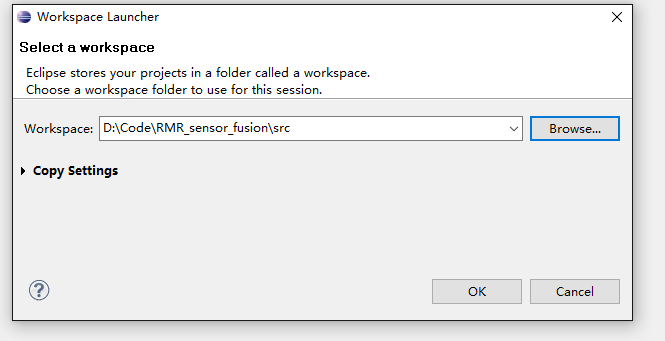
\includegraphics[width=0.5\linewidth]{fig/Note1_2}
  	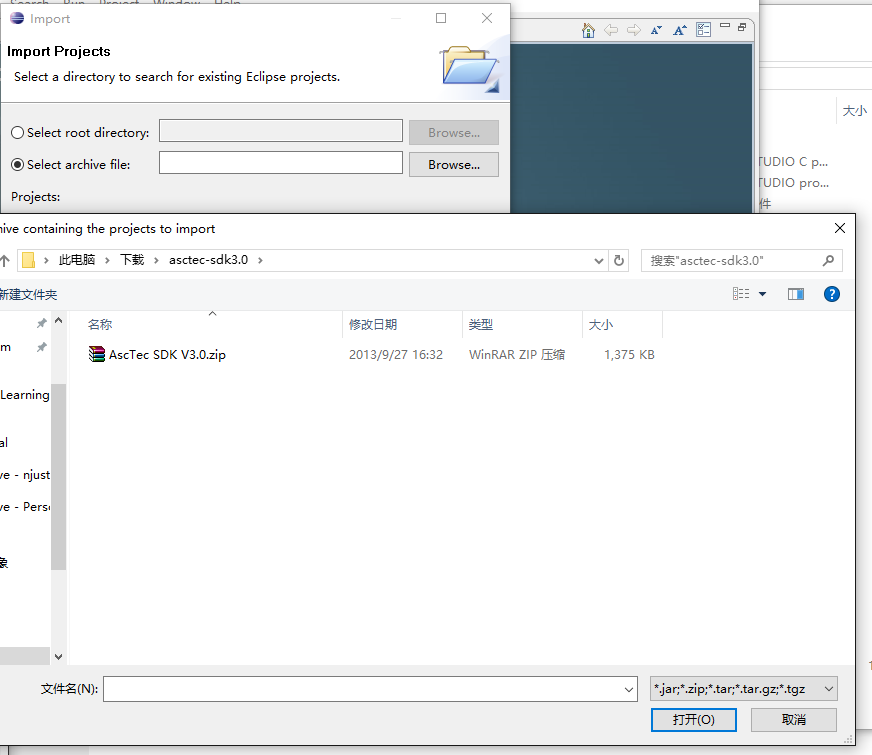
\includegraphics[width=0.5\linewidth]{fig/Note1_4}  
  	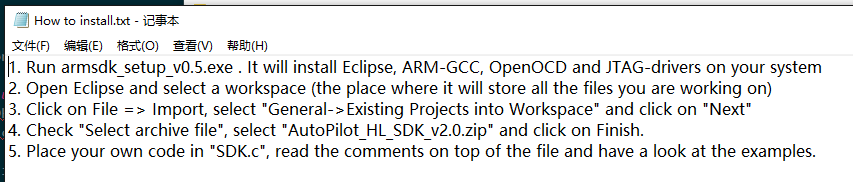
\includegraphics[width=0.9\linewidth]{fig/Note1_3}
  	\caption{Use the changed SDK code}  	
  	\label{fig:note12}
  \end{figure}
  
  
  %-----------------------------------------------
  
  \section{The Work of Project}
  112
   
  \subsection{dataset and sample}
  
   32
   23 

  

  
  
  
  \subsection{recognition}
 54645
    

  \subsection{training}
	354564
  
  
  
 
\end{document}
